\section{Прости заявки в SQL}

\subsection{Въведение}
Езикът за създаване на заявки към релационни СУБД-та е SQL (Structured Query Language).

\begin{itemize}
    \item Създават и изтриват обекти в СУБД
\begin{itemize}
    \item Бази от данни;
    \item Схеми;
    \item Потребители;
    \item Таблици и др.;
\end{itemize}
    \item Въвеждат се, променят се и се изтриват данни
    \item Извличат се данни по зададен критерии
\end{itemize}

\begin{center}
    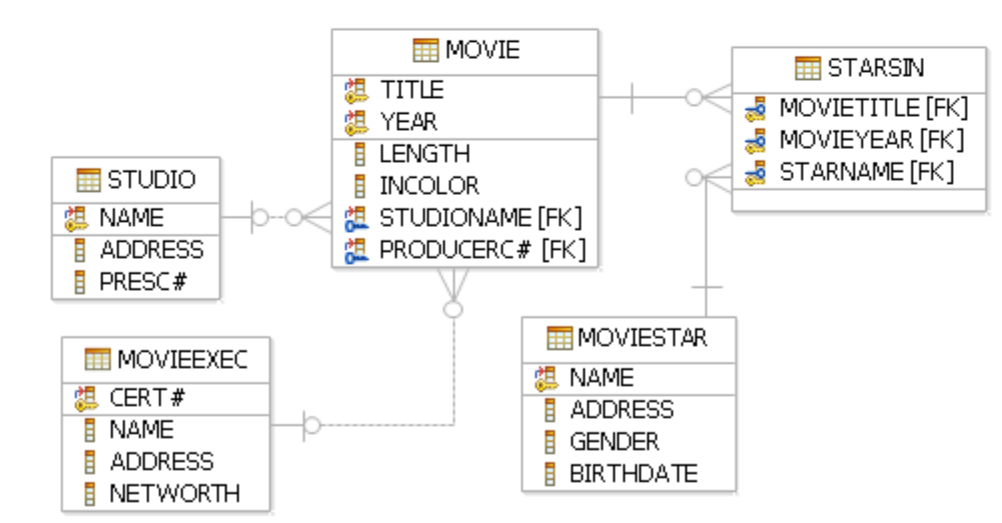
\includegraphics[width=12cm]{Movies}
\end{center}

\underline{\textbf{Примерна заявка:}}\newline
Нека ни е дадена релацията Movie (title, year, length, inColor, studionName, producerC\#).
Искаме да напишем заявка, която извежда всички филми, произведени от ‘Disney Studios’ през 1990 г.
Чрез синтаксиса на SQL, подобна заявка може да бъде написана по следният начин:

\begin{lstlisting}[language=SQL]
    SELECT *
    FROM Movie
    WHERE studioName = 'Disney' AND year = 1990
\end{lstlisting}

\begin{itemize}
    \item В FROM клаузата, се изброяват релациите към, които се отнася заявката. В нашият
    случай заявката е за релацията Movie;
    \item В WHERE клаузата, се задават условията, които трябва да бъдат удовлетворени от
    кортежите на релацията, за да отговорят на заявката. В нашият случай, условието е
    името на студиото да е ‘Disney’ и годината на филма да бъде 1990. Всички кортежи
    които отговарят едновременно на тези две условия, отговарят на критериите в
    заявката и са търсеният резултат.
    \item SELECT клаузата, задава кои атрибути на кортежите удовлетворяващи условието от
    WHERE клаузата да бъдат изведени. В нашия случай * указва, че ще бъдат изведени
    всички атрибути на кортежите.
\end{itemize}

Редът на изпълнение на горната заявка е FROM – WHERE – SELECT. Първо се определя за коя релация (релации) 
се отнася заявката и за всеки един от кортежите на тази релация се прилагат критериите от WHERE клаузата. 
За всички кортежи от релацията, които удовлетворяват критериите, се прилага и SELECT клаузата. 
Трябва да отбележим, че от гореописаната конструкция, само SELECT и FROM клаузите са задължителни, а 
WHERE клаузата е опционална.\newline
Пълният синтаксис на SQL заявка е следният:

\begin{lstlisting}[language=SQL]
    SELECT  {[DISTINCT | ALL] { * } |
            [{[schema.]{table | view}.* | expr } [AS] c_alias ]
            [,{[schema.]{table | view}.* | expr } [AS] c_alias ]...}
    
    FROM    [schema.]{table | view} [t_alias]
            [, [schema.]{table | view} [t_alias] ] ...
    
    [WHERE condition]
    [GROUP BY expr [, expr] ...
        [HAVING condition] ]
    
    [ORDER BY   {expr | position}[ASC | DESC]
                [,{expr|position}[ASC | DESC]]..]
\end{lstlisting}

\subsection{Проекция}
Елиминира част от атрибутите на извлечените кортежи.
\begin{itemize}
    \item Различни имена за атрибутите с AS
    \item Aритметични оператори и константни изрази
\end{itemize}
Пример:
\begin{lstlisting}[language=SQL]
    SELECT studioName as Name, title
    FROM Movie
\end{lstlisting}

\subsection{Селекция}
В резултатното множество попадат само тези редове, които отговарят на зададено условие.\newline
Пример:
\begin{lstlisting}[language=SQL]
    SELECT *
    FROM Movie
    WHERE studioName='Disney' AND year=1990
\end{lstlisting}

\subsection{Сравняване на низове}
Низове се сравняват:
\begin{itemize}
    \item С използване на операторите за сравнение
    \item На базата на шаблон с ключовата дума LIKE:
    \begin{itemize}
        \item s LIKE p (s – низ, p – шаблон)
        \item Шаблони – низове, в които може да се използват:
        \begin{itemize}
            \item[] \% - всякаква последователност от 0 или повече символи;
            \item[] \_ - покриване на 1 произволен символ.
        \end{itemize}
        \item Отрицанието на LIKE е NOT LIKE
    \end{itemize}
\end{itemize}

\subsection{NULL стойности}
\begin{itemize}
    \item NULL се използва за стойност на атрибутите, когато:
    \begin{itemize}
        \item Не знаем каква трябва да е стойността;
        \item Няма смислена стойност, която да зададем;
        \item Може изрично да се задава атрибутите да не могат да приемат NULL стойност;
    \end{itemize}
    \item NULL стойностите не удовлетворяват никое условие освен
    \begin{itemize}
        \item IS NULL
    \end{itemize}
    \item Резултат от сравнение:
    \begin{itemize}
        \item TRUE или FALSE
        \item Върху стойности с NULL – UNKNOWN
        \item В крайния резултат попадат само тези кортежи, за които резултатът е TRUE
    \end{itemize}
\end{itemize}

\begin{tabular}{| c | c | c | c | c |}
    \hline
    \textbf{A} & \textbf{B} & \textbf{A and B} & \textbf{A or B} & \textbf{not B} \\
    \hline
    \textbf{UNKNOWN} & \textbf{TRUE} & UNKNOWN & TRUE & FALSE \\
    \hline
    \textbf{UNKNOWN} & \textbf{UNKNOWN} & UNKNOWN & UNKNOWN & UNKNOWN \\
    \hline
    \textbf{UNKNOWN} & \textbf{FALSE} & FALSE & UNKNOWN & TRUE \\
    \hline
\end{tabular}

\subsection{Сортиране на резултата}

\begin{itemize}
    \item Резултатът от изпълнението на дадена заявка може да бъде сортиран.
    \item В SQL това се указва чрез клаузата ORDER BY
    \item ORDER BY <list of attributes or expressions> [ASC | DESC]
\end{itemize}

Например ако към горната заявка, която извежда всички филми, произведени от ‘Disney Studios’ през 1990 г., 
добавим и условието подредени по дължина и име на филм в нарастващ ред, заявката ще изглежда така:

\begin{lstlisting}[language=SQL]
    SELECT *
    FROM Movie
    WHERE studioName = 'Disney' AND year = 1990
    ORDER BY length, title ASC
\end{lstlisting}

Както се вижда от горната заявка, след клаузата ORDER BY може да стои списък от атрибути и запазената 
дума ASC, която указва, че резултатът ще бъде нареден в нарастващ ред. За подредба на резултата в 
намаляващ ред се използва запазената дума DESC. Използването на тези запазени думи е опционално. По 
подразбиране резултата се подрежда в нарастващ ред.
